%https://www.overleaf.com/latex/templates/elsevier-article-elsarticle-template/vdzfjgjbckgz

%\documentclass[preprint,12pt]{elsarticle}
%\documentclass[final,12pt,twocolumn]{elsarticle}

%% Use the option review to obtain double line spacing
%% \documentclass[authoryear,preprint,review,12pt]{elsarticle}

%% Use the options 1p,twocolumn; 3p; 3p,twocolumn; 5p; or 5p,twocolumn
%% for a journal layout:
%% \documentclass[final,1p,times]{elsarticle}
%% \documentclass[final,1p,times,twocolumn]{elsarticle}
%% \documentclass[final,3p,times]{elsarticle}
%% \documentclass[final,3p,times,twocolumn]{elsarticle}
%% \documentclass[final,5p,times]{elsarticle}
 \documentclass[final,5p,times,twocolumn]{elsarticle}

%% For including figures, graphicx.sty has been loaded in
%% elsarticle.cls. If you prefer to use the old commands
%% please give \usepackage{epsfig}

\usepackage{amsmath,amsfonts,amssymb,amsthm,mathrsfs,mathdots,mathabx,mathtools}
\usepackage{lineno}
\usepackage[english]{babel}
\usepackage{tipa}
\usepackage{geometry}
\usepackage{caption}
\usepackage{subcaption}
%\usepackage{placeins} %floatbarrier

% Hyphenation
\hyphenation{Dis-pho-nia}

\journal{Speech Communication}

\begin{document}

\begin{frontmatter}

\title{Voice quality modification using glottal pulse parameters in the WORLD vocoder}

\author[inst1]{Benjamín Opazo}
\author[inst1]{Matías Zañartu}
\ead{matias.zanartu@usm.cl}

\affiliation[inst1]{organization={Universidad Tecnica Federico Santa Maria, Electronics Department},
                addressline={Avenida Espana 1680},
                city={Valparaiso},
                postcode={2390123}, 
                country={Chile}}

\begin{abstract}
Self-perception of voice quality is a poorly understood phenomenon that is hypothesized to play a critical role in the development of hyperfunctional voice disorders.  By means of voice quality perturbation experiments altering auditory feedback, researchers could further investigate the underlying laryngeal motor control mechanisms. However, there are no synthesizers capable of altering voice quality in a physiologically relevant and controlled manner, even less so in real-time. This study introduces a Vocoder capable of altering voice quality at the glottal source level with very low latency and high quality resynthesized signals. The proposed Vocoder is built upon the well-known WORLD synthesizer by adding a Rosenberg++ pulse as glottal excitation signal with a special shape control parameter that simultaneously alters the instants of maximum excitation, maximum flow, and the return phase. In addition, methods for altering fundamental frequency, spectral envelope, and voice aperiodicity are considered.  Both perceptual and objective experiments were carried out to assess the ability of the proposed method to control voice quality. Perceptual experiments were based on a CAPE-V assessment for six simulated qualities (modal, breathy, rough, vocal fry, dysphonia) and objective experiments related the control parameters with standard measures of voice quality such as spectral tilt, cepstral peak prominence, etc. Both evaluations illustrate that the resynthesized voice is natural, physiologically accurate and that it can mimic different pathological voice qualities for vocally healthy subjects. Further efforts are needed to assess the performance of the proposed system in the opposite direction, i.e., mimicking normal voices for patients. Computational performance results show sufficiently low latency to enable future real-time implementation of the proposed Vocoder in an embedded system.
\end{abstract}

\begin{keyword}
%% keywords here, in the form: keyword \sep keyword
Voice Quality \sep Vocoder
%% PACS codes here, in the form: \PACS code \sep code
\PACS 0000 \sep 1111
%% MSC codes here, in the form: \MSC code \sep code
%% or \MSC[2008] code \sep code (2000 is the default)
\MSC 0000 \sep 1111
\end{keyword}

\end{frontmatter}

%% \linenumbers

\section{Introduction}

Auditory feedback plays an important role in speech production \cite{Elman1981}, and by modifying auditory feedback, it is possible to study the underlying mechanisms of speech motor control. A well-known example of perturbed auditory feedback is the Delayed Auditory Feedback (DAF), where a delay of $200 ms$ may induce an increase in speech errors and a decreased speech rate\cite{Chesters2015}. Auditory feedback perturbation including formant changes \cite{Tourville2008} and pitch perturbation \cite{Abur2021}\cite{Abur2020} has been used to study neurological mechanisms of voice production. The role of self-perception of voice quality has not been explored in literature and it is believed to play a critical role in the development of hyperfunctional voice disorders \cite{Galindo_2017}. 

In order to synthesize and modify voice in real-time, a specialized Vocoder is needed. Usually, Vocoders are not designed with real-time capabilities, or perform poorly in real-time conditions. An early example of a high quality real-time Vocoder is STRAIGHT\cite{Kawahara1999}, but resulting voices degrade in quality if the Vocoder is implemented in real-time, hence STRAIGHT has been phased out by more modern implementations of similar ideas such as TANDEM-STRAIGHT\cite{tandem2008}\cite{tandem2011}, which attempts to simplify the STRAIGHT Vocoder but its real-time performance is degraded with respect to the original Vocoder. The WORLD Vocoder\cite{Morise2016} is a modern Vocoder that aims to synthesize high-quality real-time voice. It is an order of magnitude faster than the STRAIGHT Vocoder and perceptually performs better than the STRAIGHT Vocoder. The Vocoder decomposes the voice signal into its fundamental frequency, spectral envelope and aperiodicity, which allows for the modification of different characteristics of voice. Using machine learning to synthesize high-quality voice in real-time is possible using Vocoders such as Vocaine \cite{vocaine}, which uses traditional Vocoders for the analysis and machine learning for the synthesis. An important shortcoming with this approach is the need for a dataset with pathological voices, and also that the subsequent trained model will probably be limited by dataset biases, such as language.

This work proposes an extension of the state-of-the-art WORLD voice Vocoder to modify voice quality of a speaker with low latency, and it also assesses the performance of the extended Vocoder in terms of voice quality, using objective and perceptual measures of voice quality.

\section{Methods}

To modify voice quality, three main tasks were performed. First, the WORLD Vocoder was extended so that it can be used to modify voice quality, then, synthetic voices were generated with modified voice quality to be evaluated both subjectively and objectively.

\subsection{Overview}

The WORLD Vocoder consists of three estimation blocks; DIO or HARVEST for the fundamental frequency estimation \cite{morise2009dio}\cite{Morise_2017harvest}, Cheaptrick for the spectral envelope estimation \cite{Morise2015cheaptrick}, and D4C for the aperiodic parameter estimation\cite{Morise2016-2}. Then, a synthesis block uses an impulse train along with the estimated parameters to synthesize natural sounding voice. To modify voice quality using the WORLD Vocoder, three modifications were done to the Vocoder; 1) The excitation signal of the synthesis part was changed from an impulse train to a Rosenberg++ (R++) \cite{Veldhuis_1998}\cite{doval2006spectrum} pulse train, 2) the spectral envelope estimation was modified so that the estimated spectrum is consistent with the new excitation signal, 3) and several modifications were applied to the parameters and variables of the Vocoder during the synthesis time to modify voice quality. Figure \ref{fig:WORLD_blocks} shows the proposed WORLD Vocoder extension, where the green blocks are modified with respect to the original implementation, and purple blocks are new proposed blocks. For synthesis, a set of parameters was created that are used to modify voice quality.
 
\begin{figure}[!htpb]
    \centerline{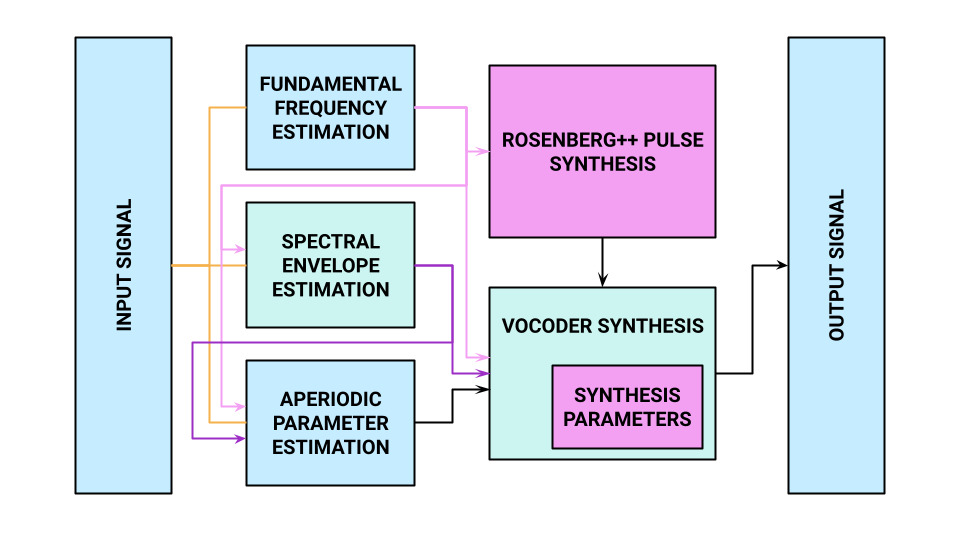
\includegraphics[width=\columnwidth]{proposed_world.jpeg}}
    \caption{\label{fig:WORLD_blocks} Proposed Extended WORLD Vocoder. Blue blocks are left unmodified, green blocks are modified with respect to the original implementation, and purple blocks are new proposed blocks. The Vocoder Synthesis block has an internal section where new parameters are defined.}
    \raggedright
\end{figure}


The Rosenberg++ pulse is controlled using a wave shape parameter known as the $R_d$ parameter \cite{fant1995lf}, which is related to the quantification of the covariance of the parameters of the Liljencrants-Fant Model, although it also works with the R++ model, where lower values of the $R_d$ parameter are related to relaxed glottal pulses and higher values are related to tighter phonation as it can be seen in Figure \ref{fig:rd_comparison}. This parameter has been successfully used to modify the breathiness of synthesized voices \cite{Degottex_2011} \cite{Degottex_2013} \cite{Murphy_2019}, but this work presents a framework capable to do it in real-time if implemented in an embedded system.

\begin{figure}[!htpb]
    \centerline{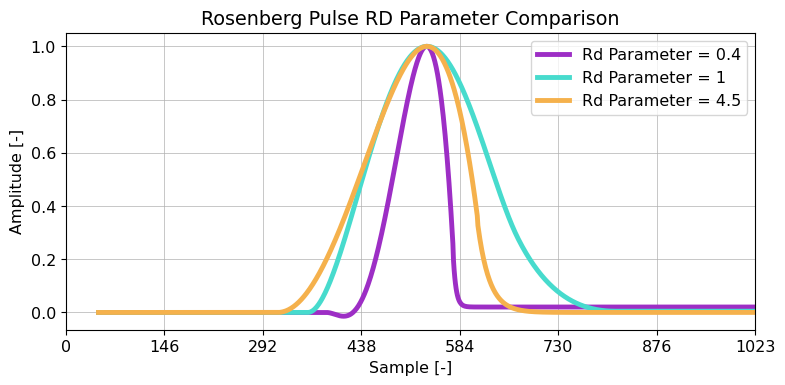
\includegraphics[width=\columnwidth]{rosenberg_rd.png}}
    \caption{\label{fig:rd_comparison}Comparison of Rosenberg++ Pulse Synthesized with different values of the $R_d$ Parameter. Lower values of the $R_d$ Parameters show a tighter pulse. When the $R_d$ parameter is lower than $0.4$, a small negative section starts appearing at the beginning of the pulse.}
    \raggedright
\end{figure}

Modal voice was also resynthesized using the R++ as an excitation signal with mixed results; while the synthesized voice still sounds natural and similar to the input signal, the resulting voices are rougher, leaving place for improvements of the modal voice synthesis. Jitter and shimmer were synthesized by modulating the frequency and amplitude of the excitation signals. To synthesize vocal fry, the fundamental frequency was lowered to the range of $50-75$ [Hz] with good results. Dysphonic voices were synthesized by lowering the amplitude of the excitation signal while maintaining lower values of the $R_d$ parameter with respect to breathy voices. Rough voice was synthesized with by slightly lowering the fundamental frequency and adding jitter and shimmer, but results were not satisfactory.

\subsection{WORLD Vocoder extension}

The original implementation of the WORLD Vocoder uses an impulse train as an excitation signal, which means that the design of the Vocoder considers it in the implementation of the spectral envelope estimation (Cheaptrick). If no modifications are made to the Cheaptrick after modifying the synthesis module, then the synthesized voice sounds muffled with the lower frequencies exacerbated. This is due to the fact that the spectral envelope that extracts Cheaptrick includes the effect of the glottal folds, which is similar to a low-pass filter, and the excitation signal using a R++ pulse works as a second cascading low-pass filter applied to the spectrum. To solve this problem, a solution is proposed where the estimated spectral envelope is modified using the following function:

\begin{equation}
    \label{eq:exppm}
    f[n] = \exp(n \frac{p}{m} - p)
\end{equation}

Where $n \leq m$ and $p$ is related to the slope of the exponential. This modifier is applied to the first $m$ samples. Note that $f[m] = 1$, so that the change between the modified spectrum and the unmodified part is smooth. The proposed modifier is applied directly to the estimated spectral envelope array frame by frame. Results shows that by tuning the $m$ and $p$ parameters it is possible to synthesize natural sounding voice that resembles the input signal.

The R++ pulse is used as an excitation signal for the synthesis module. The implementation of the R++ does not differ from the specification of the pulse \cite{Veldhuis_1998}\cite{doval2006spectrum}, except for 1) if $t_p = 2t_e/3$ or $|t_p - t_e| < 0.001$ the pulse is not synthesized, and 2) the amplitude is defined as the maximum value of the pulse at $f(t_p)$, which differs to the original implementation where the amplitude is defined as the maximum value of the derivative of the pulse. To calculate the amplitude, an internal parameter $K_{int}$ is defined as follows. If $t_a > 0$

\begin{equation}
    K_{int} =
        \begin{cases}
            3K/(t_{p}^{3}(2 t_x - t_p)) & t_p < \frac{(4D(t_0,t_e,t_a)t_a t_e + t_{e}^{2})}{(2D(t_0,t_e,t_a)t_a+t_e)} \\
            -3K/(t_{p}^{3}(2 t_x - t_p)) & \text{otherwise} \\
        \end{cases}
\end{equation}

If $t_a = 0$, then $K_{int}$ is defined as

\begin{equation}
    K_{int} =
        \begin{cases}
           3K/(t_{p}^{3}(2t_x - t_p)) & t_p < t_e \\
           -3K/(t_{p}^{3}(2t_x - t_p)) & \text{otherwise} \\
        \end{cases}
\end{equation}

To avoid a division by $0$, the restriction $|t_p - t_e| < 0.001$ is applied. With this implementation of the R++ pulse, it is possible to determine the amplitude of the pulse with the parameter $K$.

The synthesis module was extended so that it can use different parameters that allow for the modification of voice quality. The parameters that are implemented in the synthesis block are the following:

\begin{enumerate}[i)]
    \item $R_d$ Parameter: This parameter controls the $R_d$ value used to synthesize a R++ Pulse. The $R_d$ parameter is used to obtain the values of the $t_e$, $t_p$ and $t_a$ parameters of the pulse using the (COVAREP) toolbox \cite{Degottex2014_covarep}(v1.4.2), which corresponds to the instant of maximum excitation, the instant of the maximum glottal flow, and the return phase constant, respectively.
    \item $F_0$ filter frequency and order: These parameters apply a low-pass Butterworth filter to the $F_0$ array used by the Vocoder, controlling the frequency and the order of the filter.
    \item $F_0$ multiplier: This parameter is used to multiply the values of the $F_0$ array with a fixed value.
    \item Jitter Amplitude and Frequency: These parameters are used to add jitter to the voice, by modulating the array of the $F_0$ estimated values with multiplicative Brownian noise. The noise is generated by low-pass filtering white Gaussian noise with a Butterworth filter, where the Amplitude parameter refers to the power of the Gaussian noise and the Frequency parameter refers to the cutoff frequency of the low-pass filter.
    \item Shimmer Amplitude and Frequency: These parameters are used to add shimmer to the voice, by modulating the amplitude of the synthesized pulses used for the excitation signal. Like the jitter parameters, the amplitude is modulated with Brownian noise generated with the low-pass filtering of a Butterworth filter, but in this case, the noise is added. The amplitude controls the power of the white Gaussian noise and the Frequency controls the cutoff frequency of the low-pass filter.
    \item Vibrato Amplitude and Frequency: These parameters add vibrato to the $F_0$ estimated array by multiplying it with a sine wave, with an amplitude defined by the Amplitude parameter and the frequency determined by the Frequency parameter.
    \item Spectrum Filtering $p$ and $m$: This parameter controls the values of the $p$ and $m$ variables of Eq. \ref{eq:exppm}
    \item R++ $t_e$, $t_p$ and $t_a$ multiplier: These multipliers allow for a fine tuning of the $t_e$, $t_p$ and $t_a$ parameters obtained with the $R_d$ parameter. It multiplies each value with a number, modifying the values used for the synthesis of the pulse.
    \item R++ $K$ multiplier: This multiplier changes the amplitude of the synthetic R++ pulse.
    \item Band Aperiodicity Multiplier: This parameter modifies the estimated aperiodic parameter obtained by D4C in the analysis phase of the Vocoder. It multiplies the values of the aperiodic parameter for each individual frequency band that the Vocoder uses.
\end{enumerate}

\subsection{Voice quality modification: perceptual assessment}
\label{sec:perceptual}

In order to modify voice quality by adding different pathological sounds to the input signals, the Vocoder uses different parameters and values, which is highly dependant of the input voice. Table \ref{tab:vqm} shows the parameters used to synthesize different pathological voices, but not the specific values. The input signals were taken from the Perceptual Voice Quality Database \cite{pvqd}, the male signal corresponds to audio file \textit{LA\_9011\_ENSS} and the female signal to audio file \textit{LA9023\_ENSS}.

\begin{table*}[!htpb]
    \centering
    \begin{tabular}{p{0.28\textwidth} p{0.05\textwidth} p{0.05\textwidth} p{0.09\textwidth} p{0.05\textwidth} p{0.05\textwidth} p{0.05\textwidth}}
        \hline \hline
        Parameter & Modal & Breathy  & Vocal fry & Rough Voice & Dysphonia \\ \hline
        $R_d$                                   & 1 & 1 & 1 & 1 & 1 \\
        $F_0$ filter frequency and order        & 0 & 0 & 0 & 0 & 0 \\
        $F0$ multiplier                         & 0 & 0 & 1 & 1 & 0 \\
        Jitter Amplitude and Frequency          & 0 & 0 & 1 & 1 & 0 \\
        Shimmer Amplitude and Frequency         & 0 & 0 & 1 & 1 & 0 \\
        Vibrato Amplitude and Frequency         & 0 & 0 & 0 & 0 & 0 \\
        Spectrum Filtering $p$ and $m$          & 1 & 1 & 1 & 1 & 1 \\
        R++ $t_e$, $t_p$ and $t_a$ multiplier   & 1 & 1 & 1 & 1 & 1 \\
        R++ $K$ multiplier                      & 1 & 1 & 1 & 1 & 1 \\
        Band Aperiodicity Multiplier            & 0 & 1 & 0 & 0 & 1 \\ \hline \hline
    \end{tabular}
    \caption{Parameters used to synthesize modified voice quality. A $1$ means that the parameter is used and a $0$ means that the parameter is not used}
    \label{tab:vqm}
\end{table*}

A perceptual assessment task was done on the resulting voices with three expert raters using the CAPE-V evaluation tool \cite{Kempster2009} and adding two extra parameters to be evaluated: Vocal Fry and Aperiodicity.

\subsection{Voice quality modification: objective assessment}

The same two input files that are used in section \ref{sec:perceptual} are used in this experiment, with the sole difference that only two sections of the audio files are used, one where the \textipa{/A:/} utterance is said and one where the subject says "\textit{Peter will keep at the peak}".

The signals are then synthesized while modifying a single parameter in a specified range, as seen in Table \ref{tab:paramrange}. For each synthesized signal a set of objective parameters are calculated which are shown and defined in Table \ref{tab:objectexpl}.

\begin{table}[!htpb]
    \centering
    \begin{tabular}{cccc}
        \hline \hline
        \textbf{Parameter}  & \textbf{Min Value} & \textbf{Step Size} & \textbf{Max Value} \\ \hline
        $R_d$               & 0.35               & 0.05               & 4                  \\
        $F0$ multiplier     & 0.5                & 0.1                & 4                  \\
        Jitter Amplitude    & 0                  & 2                  & 50                 \\
        Jitter Frequency    & 0                  & 100                & 22000              \\
        Shimmer Amplitude   & 0                  & 2                  & 50                 \\
        Shimmer Frequency   & 0                  & 100                & 22000              \\
        R++ $K$ multiplier  & 0                  & 0.2                & 5                  \\ \hline \hline
    \end{tabular}
    \caption{Minimum, maximum and step values of the parameters}
    \label{tab:paramrange}
\end{table}

\begin{table*}[!htpb]
    \centering
    \begin{tabular}{p{0.28\textwidth} p{0.68\textwidth}}
        \hline \hline
        \textbf{Objective Measurement}                 & \textbf{Description} \\ \hline
        Cepstral Peak Prominence (CPP)                 & Measure of the cepstral peak amplitude normalized for overall amplitude \cite{Hillenbrand1994}. It is known to be a robust measure of dysphonia severity and breathy voices \cite{Fraile2014} \\
        Harmonic-to-Noise Ratio (HNR)                 &   Measure of the Ratio of the estimated harmonic component of the signal and the noise component of the signal. Note that, in order to estimate the harmonic component, an $F_0$ estimation is needed, which is not done using DIO or Harvest from the WORLD Vocoder \\
        Mean Jitter                                    & Corresponds to the pitch period deviations, calculated in 0.2 [ms] frames, and averaged across the signal\cite{opensmile}. \\
        Mean Shimmer                                   &              Corresponds to the pitch period amplitude deviations, calculated in 0.2 [ms] frames, and averaged across the signal\cite{opensmile}. \\
        Perceptual Evaluation of Speech Quality (PESQ) &        Measure used for the automated assessment of speech quality. To measure the PESQ, a python implementation was used, corresponding to the pip package PESQ V0.0.3 \\
        Peak Slope (PS)                                & Corresponds to the regression line that fits the log10 of the peaks of the time domain maxima of the signal that was previously decomposed in octaves. This parameter is used to identify breathy to tense voice qualities \cite{Kane_identifyingregions} \\
        Spectral Envelope H1-H2 (SE)                   & Corresponds to the difference in decibels (or energy ratio) of the first harmonic (H1) and second harmonic (H2). \\ \hline \hline
    \end{tabular}
    \caption{Objective measurements definitions}
    \label{tab:objectexpl}
\end{table*}

\section{Results}

Results indicate that both the perceptual and objective assessment of the synthesized signals are satisfactory. The worst performing synthetic signal in the perceptual assessment was the rough voice both for male and female subject. The objective assessment shows that the synthesis parameters are physiologically relevant.

\subsection{Voice quality modification: perceptual assessment}

Tables \ref{tab:percassmale} and \ref{tab:percassfemale} show the averaged results of the three perceptual evaluations. All synthetic voices were evaluated using the CAPE-V protocol with three expert raters.

Results show that the modal voice synthesis works as expected for the male voice, synthesizing a signal with similar CAPE-V values, whereas the female synthesis shows mildly deviant values of overall severity, roughness and aperiodicity. This means that the Vocoder needs more fine tuning for the synthesis of female voices. This suggests that the synthesized female voice using the R++ Pulse and the proposed WORLD Vocoder is not synthesizing a completely authentic voice, although in terms of the overall severity, it is the best rated voice for male and female voice, which serves as a baseline for comparison when modifying voice quality. It is worth noting that, however, the rough synthesized voice has a comparable value of overall severity for the case of female voice.

The synthesized breathy voice shows that the male voice is severely deviant, although the female voice needs more work, with a moderately deviant score for overall severity and a lower than expected value of perceived breathiness. For the dysphonic voice, results show that the synthetic voice has high values of breathiness (severely deviant), but roughness and aperiodicity are also present with moderately deviant values, and mildly deviant values of strained voice. The breathiness value for the female dysphonic synthetic voice show higher values than its breathy synthetic counterpart, and the male synthetic voice shows similar values, this indicates that breathy voice needs more fine tuning, and some characteristic of the dysphonic synthesis may be useful like lower values of the pulse amplitude. Vocal fry was successfully synthesized for both male and female voice, showing severely deviant values for the male voice and moderately deviant values for the female voice. It was not possible to synthesize severely deviant vocal fry voices for the female voice, and another method is probably needed to create a stronger effect. Rough voice was unsatisfactory, and it shows the mixed results. It was possible to synthesize mildly deviant values of roughness, but these values appear in the other synthesized voices, with higher values in the dysphonic voice, and in the case of the female voice, the dysphonic voice is severely rough, whereas the rough voice is not, which probably means that the implementation of both rough and dysphonic voices needs more tuning. In general, all voices, except for the male rough voice, show higher values of the overall severity with respect to the original voice, and even with respect to the synthetic modal voice. According to one of the expert raters, the synthesizer is working for all the evaluated voices except for the rough voice, and the modal voice needs more work.

\begin{table*}[!htpb]
    \centering
    \begin{tabular}{ccccccc}
        \hline \hline
        Label & Original & Modal & Breathy & Rough & Vocal Fry & Dysphonia\\ \hline
        Overall Severity & 12 & 7  & 53 & 17 & 33 & 73 \\
        Roughness        & 0  & 0  & 17 & 27 & 7  & 58 \\
        Breathiness      & 0  & 3  & 57 & 3  & 3  & 53 \\
        Strain           & 8  & 0  & 12 & 17 & 25 & 38 \\
        Pitch            & 0  & 0  & 0  & 0  & 20 & 0  \\
        Loudness         & 0  & 0  & 10 & 0  & 10 & 17 \\
        Vocal Fry*       & 12 & 10 & 3  & 23 & 70 & 0  \\
        Aperiodicity*    & 12 & 10 & 13 & 30 & 30 & 43 \\ \hline \hline
    \end{tabular}
    \caption{Averaged CAPE-V results of the original and synthesized signals of the male subject}
    \label{tab:percassmale}
\end{table*}

\begin{table*}[!htpb]
    \centering
    \begin{tabular}{ccccccccccccc}
        \hline \hline
        Label & Original & Modal & Breathy & Rough & Vocal Fry & Dysphonia\\ \hline
        Overall Severity & 3 & 20 & 40 & 33 & 43 & 60 \\
        Roughness        & 0 & 10 & 30 & 30 & 20 & 60\\
        Breathiness      & 0 & 3  & 27 & 20 & 23 & 50\\
        Strain           & 0 & 7  & 13 & 17 & 20 & 23\\
        Pitch            & 0 & 0  & 0  & 0  & 33 & 0 \\
        Loudness         & 0 & 0  & 7  & 0  & 17 & 0 \\
        Vocal Fry*       & 0 & 0  & 0  & 17 & 40 & 0 \\
        Aperiodicity*    & 7 & 20 & 13 & 33 & 23 & 37\\ \hline \hline
    \end{tabular}
    \caption{Averaged CAPE-V results of the original and synthesized signals of the female subject}
    \label{tab:percassfemale}
\end{table*}

\subsection{Voice quality modification: objective assessment}

In accordance with the perceptual results and literature \cite{Fraile2014}\cite{HemanAckah2002}\cite{Kane_identifyingregions}\cite{Kreiman2014}, Figure \ref{fig:results_rd_cpp} shows that CPP is $6 [dB]$ lower when the $R_d$ parameter has high values, Figure \ref{fig:results_rd_se} shows that the spectral envelope varies from $10$ to $40 [dB]$, and in Figure \ref{fig:results_rd_ps}, the peak slope varies from $-0.5$ to $-0.4$. All these values indicate that the voice is changing from tense to breathy. Results of measured PESQ show that in general, higher values of the $R_d$ parameter synthesize a more different voice with respect to the original signal. It can be noted that for lower values of the $R_d$ parameter, the female sustained signal has values of over 4 in the PESQ measurements. As expected, the other parameters do not show correlations to the $R_d$ parameter.

\begin{figure*}[!htpb]
	\makebox[\linewidth][c]{
	\begin{subfigure}[b]{.49\textwidth}
		\centering
		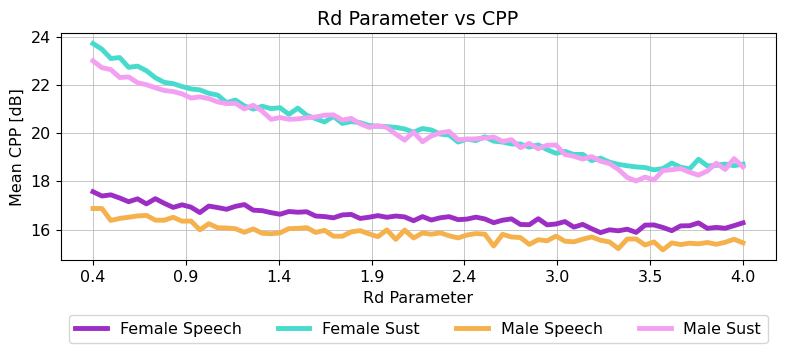
\includegraphics[width=.98\textwidth]{rd_cpp.png}
		\caption{$R_d$ Parameter vs Mean CPP}
		\label{fig:results_rd_cpp}
	\end{subfigure}
	\begin{subfigure}[b]{.49\textwidth}
		\centering
		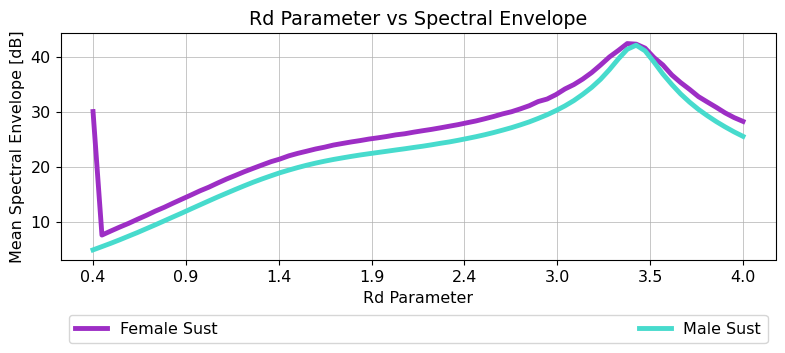
\includegraphics[width=.98\textwidth]{rd_se.png}
		\caption{$R_d$ Parameter vs Spectral Envelope}
        \label{fig:results_rd_se}
	\end{subfigure}
	}
	\\
	\makebox[\linewidth][c]{
	\begin{subfigure}[b]{.49\textwidth}
		\centering
		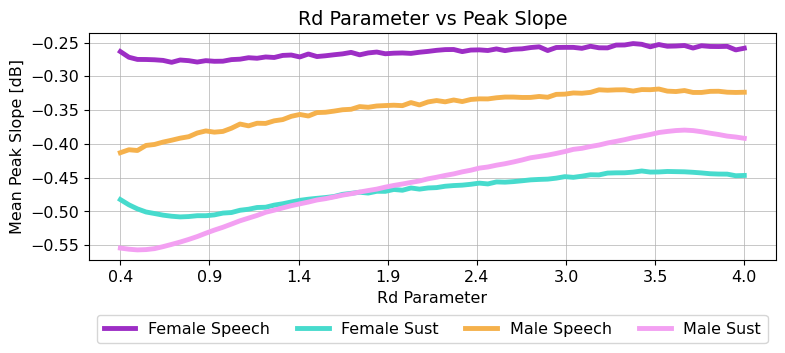
\includegraphics[width=.98\textwidth]{rd_ps.png}
		\caption{$R_d$ Parameter vs Peak Slope}
        \label{fig:results_rd_ps}
	\end{subfigure}
	\begin{subfigure}[b]{.49\textwidth}
		\centering
		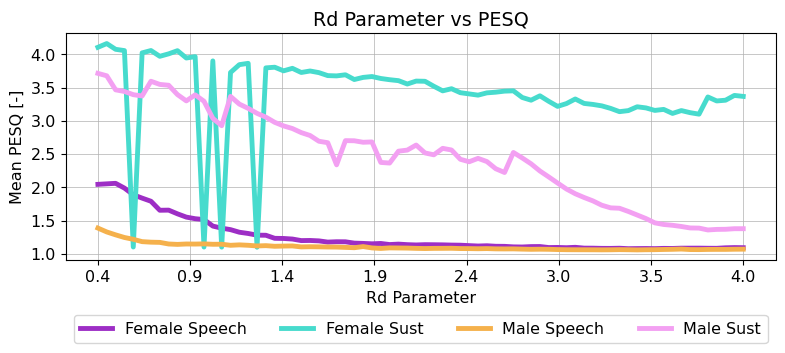
\includegraphics[width=.98\textwidth]{rd_pesq.png}
		\caption{$R_d$ Parameter vs Peak Slope}
        \label{fig:results_rd_pesq}
	\end{subfigure}
	}
	\caption{$R_d$ Parameter results}
\end{figure*}

It is clear from Figure \ref{fig:results_f0_multiplier_pesq} that the peak value of the PESQ is when the F0 multiplier is 1, which is consistent to the idea that not modifying the fundamental frequency allows for a voice that is perceptually similar to the original voice. It is important to note that this happens with all four signals, and that the peak values are similar to the peak values of Figure \ref{fig:results_rd_pesq}. This is an important result because when the F0 multiplier is 1, the Vocoder is not modifying in any aspect the voice, which means that the synthesized voice with the $R_d$ parameter can synthesize modal voice like the input signal. The other measurements are not necessarily related to the parameter, even though the results of Figure \ref{fig:results_f0_multiplier_ps} are attention grabbing, in the sense that there is a strong correlation with the PS, this could be a spurious correlation. Figure \ref{fig:results_f0_multiplier_hnr} shows that HNR is correlated with the multiplier. This is probably related to the specific implementation of the HNR, although this could not be checked because the details of the implementation of this parameter are not publicly available. The parameter is not related to the CPP as expected, however, there is a steep drop in the value in the female sustained vowel when the parameter is over 2.2.

\begin{figure*}[!htpb]
	\makebox[\linewidth][c]{
	\begin{subfigure}[b]{.49\textwidth}
		\centering
		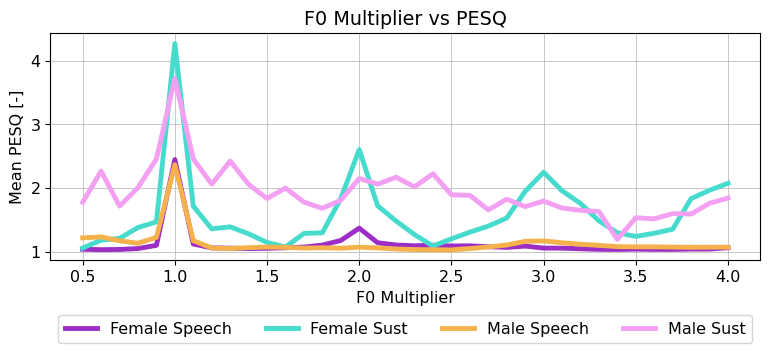
\includegraphics[width=.98\textwidth]{f0_multiplier_pesq.png}
		\caption{F0 Multiplier vs PESQ}
		\label{fig:results_f0_multiplier_pesq}
	\end{subfigure}
	\begin{subfigure}[b]{.49\textwidth}
		\centering
		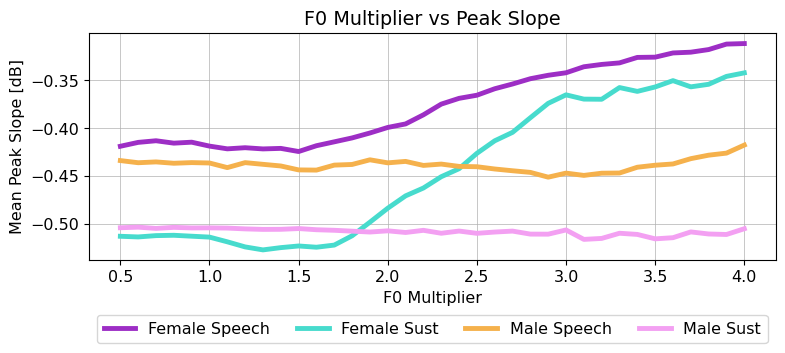
\includegraphics[width=.98\textwidth]{f0_multiplier_ps.png}
		\caption{F0 Multiplier vs Peak Slope}
        \label{fig:results_f0_multiplier_ps}
	\end{subfigure}
	}
	\\
	\centering
	\begin{subfigure}[b]{.49\textwidth}
		\centering
		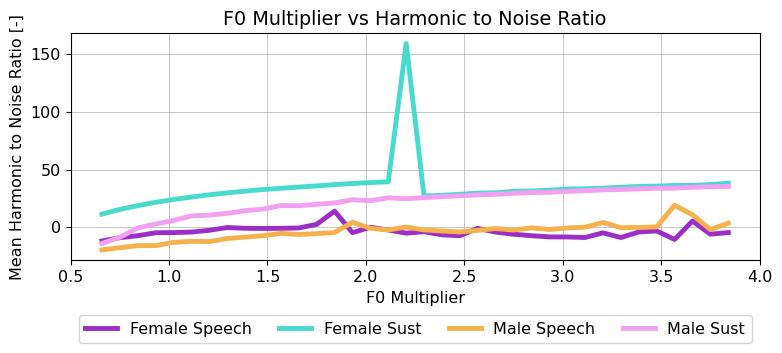
\includegraphics[width=.98\textwidth]{f0_multiplier_hnr.png}
		\caption{F0 Multiplier vs HNR}
        \label{fig:results_f0_multiplier_hnr}
	\end{subfigure}
	\begin{subfigure}[b]{.49\textwidth}
		\centering
		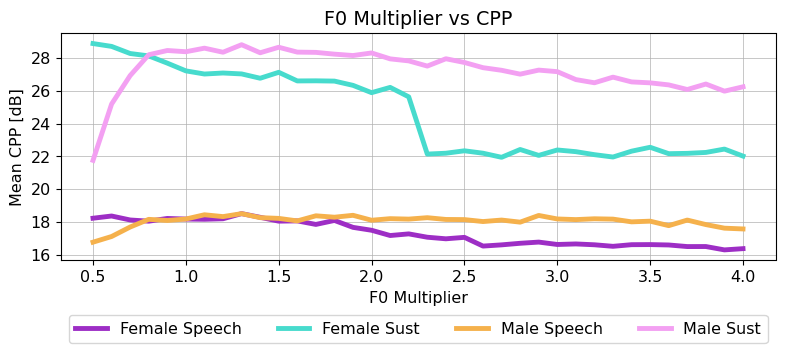
\includegraphics[width=.98\textwidth]{f0_multiplier_cpp.png}
		\caption{F0 Multiplier vs CPP}
        \label{fig:results_f0_multiplier_cpp}
	\end{subfigure}
	\caption{F0 Multiplier Parameter results}
\end{figure*}

In Figure \ref{fig:results_rpp_k_cpp} it can be noted the drastic change of the CPP of $6 [dB]$ in the case of the sustained vowels when the pulse amplitude changes from 0 to a higher value. This change is due to the fact that when this parameter is 0, there is no excitation pulse, and the synthesized signal is excited only by noise, emulating a breathy or dysphonic voice. It can be seen that this drastic change is repeated in Figure \ref{fig:results_rpp_k_pesq}, showing that when an excitation signal is present, the synthesized signal is closer to the input signal. The other parameters show a quick convergence to their maximum when R++ K multiplier parameter is greater than 0, with the exception of the measured jitter and shimmer, which is expected.

\begin{figure*}[!htpb]
	\makebox[\linewidth][c]{
	\begin{subfigure}[b]{.49\textwidth}
		\centering
		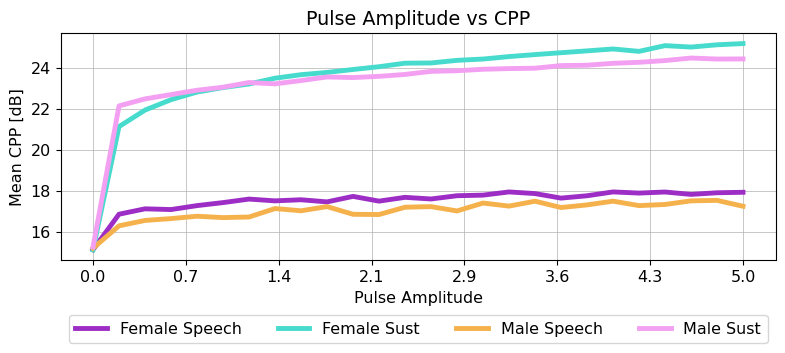
\includegraphics[width=.98\textwidth]{rpp_k_cpp.png}
		\caption{F0 Multiplier vs CPP}
		\label{fig:results_rpp_k_pesq}
	\end{subfigure}
	\begin{subfigure}[b]{.49\textwidth}
		\centering
		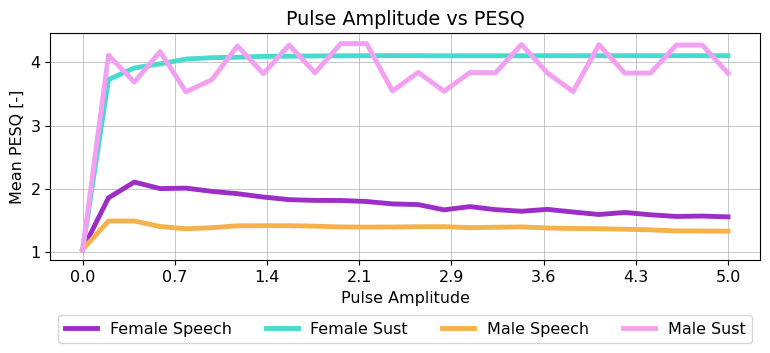
\includegraphics[width=.98\textwidth]{rpp_k_pesq.png}
		\caption{F0 Multiplier vs PESQ}
        \label{fig:results_rpp_k_cpp}
	\end{subfigure}
	}
	\caption{R++ K Multiplier Parameter results}
\end{figure*}

As expected, PESQ lowers when either the amplitude or the frequency of the jitter increases, being more susceptible to changes in frequency. The measured value of the jitter increases from $0.35\%$ to $31\%$ for changes in frequency (Figure \ref{fig:results_jitter_frequency_jitter}) and from $1.2\%$ to $25\%$ for changes in amplitude (Figure \ref{fig:results_jitter_amplitude_jitter}), which is consistent with the values of the variation of parameters. The measured shimmer is also affected in a similar manner which is unexpected, although it is probably related to how the algorithm was implemented, where it shows mixed sensitivities with respect to jitter and shimmer. The amplitude and frequency of jitter are inversely correlated with the HNR, which is what is expected, as higher values of jitter are related with a lower harmonic component of the signal. On the other hand, the Shimmer Amplitude parameter and Shimmer Frequency parameter affect the measured shimmer as it is shown in Figures \ref{fig:results_shimmer_amplitude_shimmer} and \ref{fig:results_shimmer_frequency_shimmer}, changing from $2.5\%$ to $30\%$ for changes in frequency and from $1.4\%$ to $12\%$ for changes in amplitude, which is consistent with the values of the parameters. Following a similar behaviour with respect to the 'Jitter Frequency parameter' and 'Jitter Amplitude parameter' parameters, the measured jitter for both amplitude and frequency of shimmer is affected. As expected, the PESQ values drop from near 4 to 1 when the 'Jitter Amplitude parameter' and 'Jitter Frequency parameter' parameters are higher.

\begin{figure*}[!htpb]
	\makebox[\linewidth][c]{
	\begin{subfigure}[b]{.49\textwidth}
		\centering
		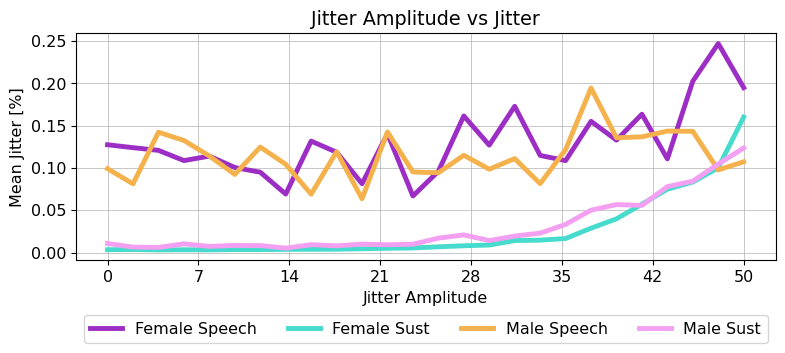
\includegraphics[width=.98\textwidth]{jitter_amplitude_jitter.png}
		\caption{Jitter Amplitude vs Mean Jitter}
		\label{fig:results_jitter_amplitude_jitter}
	\end{subfigure}
	\begin{subfigure}[b]{.49\textwidth}
		\centering
		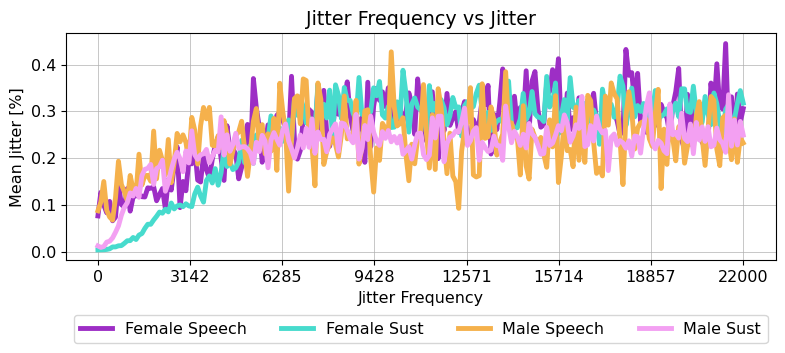
\includegraphics[width=.98\textwidth]{jitter_frequency_jitter.png}
		\caption{Jitter Frequency vs Mean Jitter}
        \label{fig:results_jitter_frequency_jitter}
	\end{subfigure}
	}
	\\
	\makebox[\linewidth][c]{
	\begin{subfigure}[b]{.49\textwidth}
		\centering
		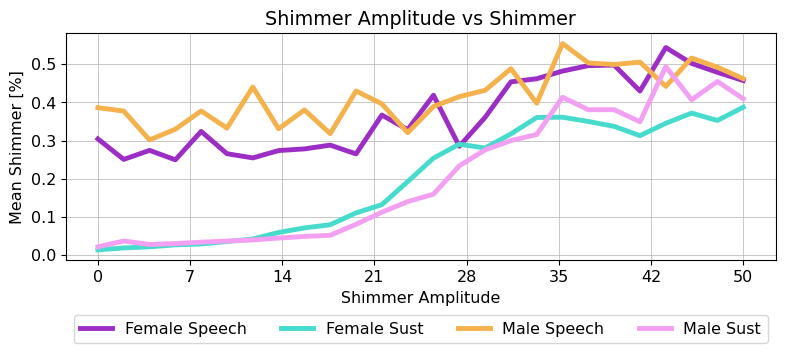
\includegraphics[width=.98\textwidth]{shimmer_amplitude_shimmer.png}
		\caption{Shimmer Amplitude vs Mean Shimmer}
		\label{fig:results_shimmer_amplitude_shimmer}
	\end{subfigure}
	\begin{subfigure}[b]{.49\textwidth}
		\centering
		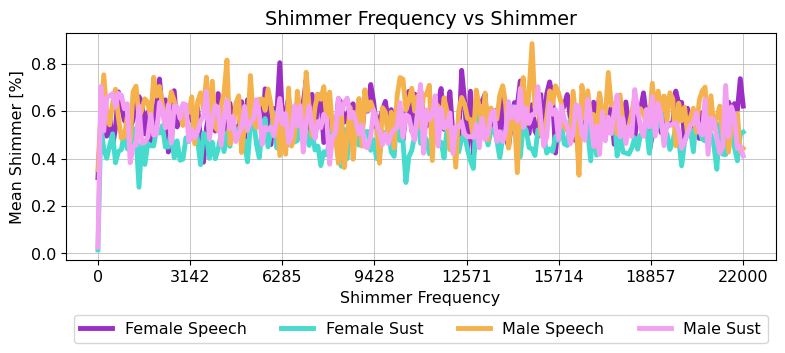
\includegraphics[width=.98\textwidth]{shimmer_frequency_shimmer.png}
		\caption{Shimmer Frequency vs Mean Shimmer}
        \label{fig:results_shimmer_frequency_shimmer}
	\end{subfigure}
	}
	\caption{Jitter and Shimmer (Amplitude and Frequency) Parameter results}
\end{figure*}

\section{Conclusion}

%Self-perception of voice quality is a poorly understood phenomenon that is hypothesized to play a critical role in the development of hyperfunctional voice disorders.  By means of voice quality perturbation experiments altering auditory feedback, researchers could further investigate the underlying laryngeal motor control mechanisms. However, there are no synthesizers capable of altering voice quality in a physiologically relevant and controlled manner, even less so in real-time. This study introduces a Vocoder capable of altering voice quality at the glottal source level with very low latency and high quality resynthesized signals. The proposed Vocoder is built upon the well-known WORLD synthesizer by adding a Rosenberg++ pulse as glottal excitation signal with a special shape control parameter that simultaneously alters the instants of maximum excitation, maximum flow, and the return phase. In addition, methods for altering fundamental frequency, spectral envelope, and voice aperiodicity are considered.  Both perceptual and objective experiments were carried out to assess the ability of the proposed method to control voice quality. Perceptual experiments were based on a CAPE-V assessment for six simulated qualities (modal, breathy, rough, vocal fry, dysphonia) and objective experiments related the control parameters with standard measures of voice quality such as spectral tilt, cepstral peak prominence, etc. Both evaluations illustrate that the resynthesized voice is natural, physiologically accurate and that it can mimic different pathological voice qualities for vocally healthy subjects. Further efforts are needed to assess the performance of the proposed system in the opposite direction, i.e., mimicking normal voices for patients. Computational performance results show sufficiently low latency to enable future real-time implementation of the proposed Vocoder in an embedded system.


In this study, it was shown that it is possible to extend the WORLD Vocoder to modify voice quality in a physiologically relevant way. The R++ pulse was introduced as an physiologically relevant excitation signal with a special shape control parameter that simultaneously altered the instants of maximum excitation, maximum flow, and the return phase. In order to introduce this new and physiologically relevant excitation signal, core components of the WORLD Vocoder were adapted. In addition to the pulse shape, several source control parameters were included to account for other temporal variations. The resulting method combining these parameters allowed for altering voice quality to mimic breathiness, dysphonia, and vocal fry. 

The perceptual relevance of the resulting synthesized signals was assessed using the CAPE-V framework. The proposed scheme was able to produce modal, breathy, dysphonia, and vocal fry qualities with good perceptual quality. However, the rough voice quality sounded less natural and its results are not perceptually satisfactory. Further work is needed to describe rough voice quality and to extend the vocoder to improve this performance. In general, the Vocoder exhibits a lower perceptual quality with female voices. Considering the multidimensional aspect of Voice Quality, it is difficult to completely isolate the effect of a given label of voice quality with a unique transformation. Our results show that the proposed methods affect more than one component of Voice Quality, even when the objective is to modify only one. For example, dysphonic synthethic voices are associated with higher values of roughness, strain and aperiodicity, even when only the amplitude of the excitation pulse was modified.

The objective evaluation of the synthesized voices provided insights on the performance of the proposed parameters. The pulse shape parameter $R_d$ yielded results that are in agreement with the literature, following the expected trends from CPP, PS, SE and PESQ. The $F_0$ multiplier was the main factor when synthesizing vocal fry and rough voices. The pulse amplitude had a clear effect on CPP and PESQ and was a key parameter to synthesize dysphonic voices. Changes in voice quality using jitter and shimmer showed relatively good performance in terms of the objective measures (mean jitter, mean shimmer), although its perceptual relevance was lower. In general, all parameters affect the resulting PESQ, which means that modifications are being made to the voice, although, each parameter perturbs differently the synthesized voice, affecting with different degrees the value of PESQ.

Note that experiments with sustained vowels showed clear trends of voice quality changes that are well aligned with the expected outcomes in the objective measures according to the literatyre. Even though they tend to have a more natural sound, experiments with running speech do not always agree with these trends. This is rather expected because the objective measurements are designed for sustained vowels, and in running speech the parameters are averaged between (sometimes drastically) different frames. In the case of the perceptual setup, the opposite effect is seen: When listening to running speech, the small imperfections of the synthesis remain unnoticed, whereas with sustained vowels, the imperfections of the synthesis are more easily noticed.

The modification of the Cheaptrick algorithm in the WORLD Vocoder allows to use different excitation signals. In this work only the R++ signal was used, but other glottal pulses could be considered, although with further modifications to the Cheaptrick algorithm. Another shortcoming of this work is that, at the moment, it is only possible to degrade voice quality rather than improve it. Future work could explore training a deep learning framework to change the estimated spectral envelope, and thus fixing vocal quality, as seen in Text-To-Speech synthesizers\cite{mozillatts} and voice separation schemes\cite{Blaauw2017} that use the WORLD Vocoder.

The proposed parameters are probably insufficient for the modification of all kinds of voice quality, although the proposed framework allow for further development in this area. Fine tuning the algorithms associated with the parameters and proposing new parameters can lead to better results of voice quality modification. Nevertheless, the proposed vocoder provides a framework for future investigation of real-time modification of voice quality in an embedded system and laryngeal motor control experiments.

%\FloatBarrier

\section{Acknowledgments}

This study was funded by ANID through grants BASAL FB0008 and FONDECYT 1191369. We acknowledge the Speech Language Pathologists Christian Castro, Diego Romero and Alejandro Herrera, who performed the perceptual CAPE-V assessments.

\bibliographystyle{elsarticle-num-names} 
\bibliography{bibliography.bib}

\end{document}
\endinput
